\subsection{Threaded joints verification}
\subsubsection*{Preliminary design}
Given the customer's requirements, the threaded fasteners used for the threaded joints in the whole robot are chosen to be standard screws with diameter of $8mm$, compatible with the $40mm$ T-slot profiles.

Considering the threaded joints present on the robot, the maximum thickness of the members is given by the sum between the beam cross section's width, $40 mm$, and the machined gussets thickness, $8 mm$. Given that two screws must fit, as in section $A$, the length of the screws is chosen to be equal to $18 mm$, according to \texttt{UNI ISO 888}; table \ref{tab:boltchoise} reports the main properties of the chosen bolt used for the verification of the connections.

\begin{table}[h!]
	\rule{\linewidth}{2pt}
	\caption{selected bolt chosen from the Parker IPS catalogue \cite{parker-ds} and related main properties.}
	\label{tab:boltchoise}
	\rule{\linewidth}{1pt} 
	\begin{center}
	\begin{tabular}{r c c}
		Parameter & symbol & value \\ \hline
		diameter & $d$ & $8mm$ \\
		head diameter & $d_0$ & $14mm$ \\
		length & $l$ & $18mm$ \\
		cross-section & $A_b$ & $16\pi mm^2$ \\
		tensile cross-section & $A_{bt}$ & $36.6mm^2$ \\
		ultimate tensile strength & $\sigma_{uts}$ & $505MPa$ \\
		product code & \multicolumn{2}{c}{\texttt{24-118-8}}
	\end{tabular}
	\end{center}
	\rule{\linewidth}{2pt}
\end{table}

With reference to Figure \ref{fig:freebodydiagramframe}, threaded joints are present in sections $A$, $B$, $C$ and $D$. The verifications are carried out with respect to the most critical sections which, according to the load analysis performed previously, are identified as section $A$ and $D$. Moreover, since the load distribution depends on the position of the point of application of the external load, the most critical condition corresponds to the one in which the load is applied in $\zeta = 1$ for section $A$ and $\zeta = 3$ for section $D$.\\
\subsubsection*{Section A}
The loads applied on section $A$ are the following:\\
\begin{itemize}
	\item axial load $N_{A} = -251.126 N$;
	\item bending moment $M_{xA} = -12.645 N\cdot m$; 
	\item bending moment $M_{yA} = 1.894 N\cdot m$; 
	\item torque $M_{zA} = -0.594 N\cdot m$.
\end{itemize}
In correspondence of section $A$, there are two machined gussets chosen from the Parker IPS catalogue \cite{parker-ds}, reported in figure \ref{fig:gusset}.
Given the geometry of the component, the threaded joints are positioned on the vertical $z$ and horizontal $x$ global axis.  For this reason, two separated analysis are performed. 
\begin{SCfigure}[1.5][bht]
	\centering
	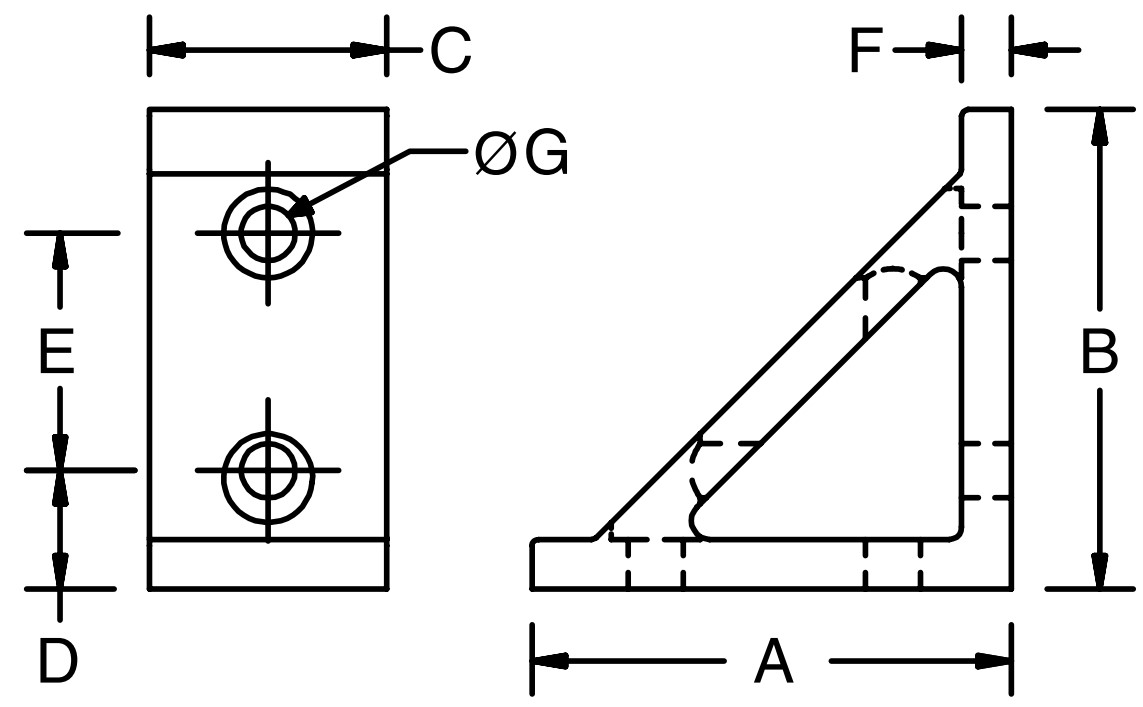
\includegraphics[width=5cm]{gusset.jpg}
	\caption{machined gusset, code \texttt{10-102}, from the IPS catalogue \cite{parker-ds}. In the drawing: $A = 77mm$, $B=77mm$, $C = 34mm$, $D= 20mm$, $E=40mm$, $F=8mm$, $G=9mm$.}
	\label{fig:gusset}
\end{SCfigure}

\paragraph{Threaded joints along the $x$ axis} The sliding actions are given by the torque $M_{zA}$, which produces a shear force on every screw equal to:\\
\begin{equation*}
    V_{i} = \frac{M_{z1}r_{i}}{\sum\limits_{i=1}^{n_{{b}}} r^2_{i}}
\end{equation*}
where $r_{i}$ are the distances of every screw from the center of the section O, and are equal to $r_{1} = 40 mm$, $r_{2} = 80 mm$. 
The shear force is calculated for the most critical screws, distant $r_{2}$ from O, and it is equal to:\\
\begin{equation*}
    V_{2} = \frac{M_{zA}r_{2}}{2r^2_{1}+2r^2_{2}} = - 2.970 N
\end{equation*}
The shear and punching resistance verifications can be performed as follow:
\begin{itemize}
    \item shear resistance verification:
    \begin{equation*}
        |V_{2}| < \frac{\sigma_{uts}A_{b}}{\phi}
    \end{equation*}
    where $\sigma_{uts}$ corresponds to the screw's ultimate tensile strength, $A_{b}$ to the bolt cross-section and $\phi$ is the safety factor which, according to Eurocode3, is equal to $\frac{1.25}{0.58}$.
    As a consequence, it follows that:
    \begin{equation*}
       \sigma_{uts} > \frac{|V_{2}|\phi}{A_{b}} = 0.127 MPa
    \end{equation*}\\
    \item crushing resistance verification:
    \begin{equation*}
        |V_{2}| < \frac{\sigma_{uts,m}dt}{\phi}
    \end{equation*}
    where $\sigma_{uts,m}$ corresponds to the member's ultimate tensile strength, $d$ to the bolt diameter and $\phi$ is the safety factor which, according to Eurocode3, is equal to 0.5. Finally, $t$ corresponds to the member's thickness, which can be calculated as the sum of the machined gusset thickness, $F = 8 mm$, and the base's thickness, equal to $16 mm$:
     \begin{equation*}
       \sigma_{uts,m} > \frac{|V_{2}|\phi}{dt} = 7.734 \cdot 10^{-3} MPa
    \end{equation*}
\end{itemize}
Separating actions are given by the axial load and the bending moments.\\
Assuming that the members are rigid it is possible to calculate the effects of the separating actions in both $xz$ and $yz$ planes.\\
The load caused by the separating action, acting on each bolt can be calculated as:\\
\begin{equation*}
    N_{i} = \frac{M_{b}h_{i}}{\sum\limits_{i=1}^{n_{b}} h^2_{i}} + \frac{N}{n_{b}}
\end{equation*}
Considering the $xz$ plane and assuming that the pivot is placed on the edge of the section, the constant $     h_{i}$ will be equal to:
\begin{equation*}
   \begin{cases}
    h_{1} = 17 mm\\
    h_{2} = 57 mm\\
    h_{3} = 137 mm\\
    h_{4} = 177 mm\\
    \end{cases} 
\end{equation*}
The normal load is calculated for the most critical screw as follow:\\
\begin{equation*}
    N_{xz} = \frac{M_{yA}h_{4}}{h_{1}^{2}+h_{2}^{2}+h_{3}^{2}+h_{4}^{2}} + \frac{N_{1}}{n_{b}} = - 56.530 N
\end{equation*}
Since the axial load acting on every bolt is negative, i.e. the bolt are subjected to compression, there are no issues relative to tension and punching resistance. As a consequence, it is not necessary to perform those verifications. \textbf{(???)}

Considering the $yz$ plane and assuming that the pivot is placed on the edge of the section, the constants $h_{i}$ will be all equal to $h = \frac{C}{2} = 17 mm$.
The normal load is equal to:
\begin{equation*}
    N_{yz} = \frac{M_{xA}h}{4h^{2}} + \frac{N_{1}}{n_{b}} = 123.175 N
\end{equation*}
The tension resistance and punching verification can be performed as follow:
\begin{itemize}
    \item tension resistance verification:
    \begin{equation*}
        N_{yz} < \frac{\sigma_{uts}A_{bt}}{\phi}
    \end{equation*}
    Where $\sigma_{uts}$ corresponds to the screw's ultimate tensile strength, $A_{bt}$ to the bolt tensile cross-section and $\phi$ is the safety factor which, according to Eurocode3, is equal to $\frac{1.25}{0.9}$. As a consequence, it follows that:
    \begin{equation*}
       \sigma_{uts} > \frac{N_{yz}\phi}{A_{bt}} = 4.674MPa
    \end{equation*}
    \item punching resistance verification:
    \begin{equation*}
        N_{yz} < \frac{\pi d_{0} t \sigma_{uts,m}}{\phi}
    \end{equation*}
    Where $\sigma_{uts,m}$ corresponds to the member's ultimate tensile strength, $d_{0}$ the bolt head diameter and $\phi$ is the safety factor which, according to Eurocode3, is equal to $\frac{1.25}{0.6}$. Finally, $t$ corresponds to the member's thickness, which can be calculated as the sum of the gusset's thickness, $F = 8 mm$, and the base's thickness, equal to $16 mm$:
     \begin{equation*}
       \sigma_{uts,m} > \frac{N_{yz}\phi}{\pi d_{0}t} = 0.243 MPa
    \end{equation*}
\end{itemize}

\paragraph{Threaded joints along the $z$ axis} In this case the sliding actions are given by $M_{xA}$ and $N_A$ which produce a shear force on every screw equal to:
\begin{equation*}
    V_{i} = \frac{M_{xA}r_{i}}{\sum\limits_{i=1}^{n_{{b}}} r^2_{i}} + \frac{N_{A}}{n_{b}}
\end{equation*}
where $r_{i}$ are the distances of every screw from the center of the section O, and are equal to $r = \frac{E}{2} = 20 mm$.
\begin{equation*}
    V = \frac{M_{xA}r}{2r^2} +  \frac{N_{A}}{2} = 140.412 N
\end{equation*}
\begin{itemize}
    \item shear resistance verification:
    \begin{equation*}
       \sigma_{uts} > \frac{V\phi}{A_{b}} = 6.20 MPa
    \end{equation*}
    \item crushing resistance verification:
     \begin{equation*}
       \sigma_{uts,m} > \frac{V\phi}{dt} = 0.183 MPa
    \end{equation*}
\end{itemize}

The separating actions, $M_{yA}$ and $M_{zA}$ generates normal load on each and the effects are studies as previously for yz and xy plane.
\begin{equation*}
    N_{i} = \frac{M_{b}h_{i}}{\sum\limits_{i=1}^{n_{b}} h^2_{i}} + \frac{N}{n_{b}}
\end{equation*}
Considering the $yz$ plane and assuming that the pivot is placed on the edge of the section, the constants $h_{i}$ will be equal to $h_1 = D = 20 mm$ and $h_2 = D + E = 60 mm$.
The normal load is evaluated for the most critical screw and is equal to:
\begin{equation*}
    N_{xz} = \frac{M_{yA}h_{2}}{h_{1}^{2}+h_{1}^{2}} = 28.404 N
\end{equation*}
\begin{itemize}
    \item tension resistance verification:
     \begin{equation*}
       \sigma_{uts} > \frac{N_{yz}\phi}{A_{bt}} = 1.078 MPa
    \end{equation*}
    \item punching resistance verification:
     \begin{equation*}
       \sigma_{uts,m} > \frac{N_{yz}\phi}{\pi d_{0}t} = 27.459 \cdot 10^{-3} MPa
    \end{equation*}
\end{itemize}
Finally, considering the xy plane, assuming that the pivot is placed on the edge of the section, the constants $h_{i}$ will be all equal to $h = \frac{C}{2} = 17 mm$ the normal load is equal to: \\
\begin{equation*}
    N_{xy} = \frac{M_{zA}h}{2h^{2}} = 17.470 N
\end{equation*}
\begin{itemize}
    \item tension resistance verification:
     \begin{equation*}
       \sigma_{uts} > \frac{N_{xy}\phi}{A_{bt}} = 0.663 MPa.
    \end{equation*}
    \item punching resistance verification:
     \begin{equation*}
       \sigma_{uts,m} > \frac{N_{xy}\phi}{\pi d_{0}t} = 16.888 \cdot 10^{-3} MPa.
    \end{equation*}
\end{itemize}

\subsubsection*{Section D}
The loads applied on section $D$ are the following:
\begin{itemize}
	\item axial load $N_{D} = 233.010 N$;
	\item bending moment $M_{xD} = 0 N\cdot m$; 
	\item bending moment $M_{yD} = 8.106 N\cdot m$; 
	\item torque $M_{zD}x = -0.594 N\cdot m$.
\end{itemize}
In correspondence of section $D$, there is a pivot joint chosen from the Parker IPS catalogue \cite{parker-ds}, reported in figure \ref{fig:pivot}.
\begin{figure}[h!]
    \centering
    \begin{subfigure}{0.32\linewidth}
    	\centering 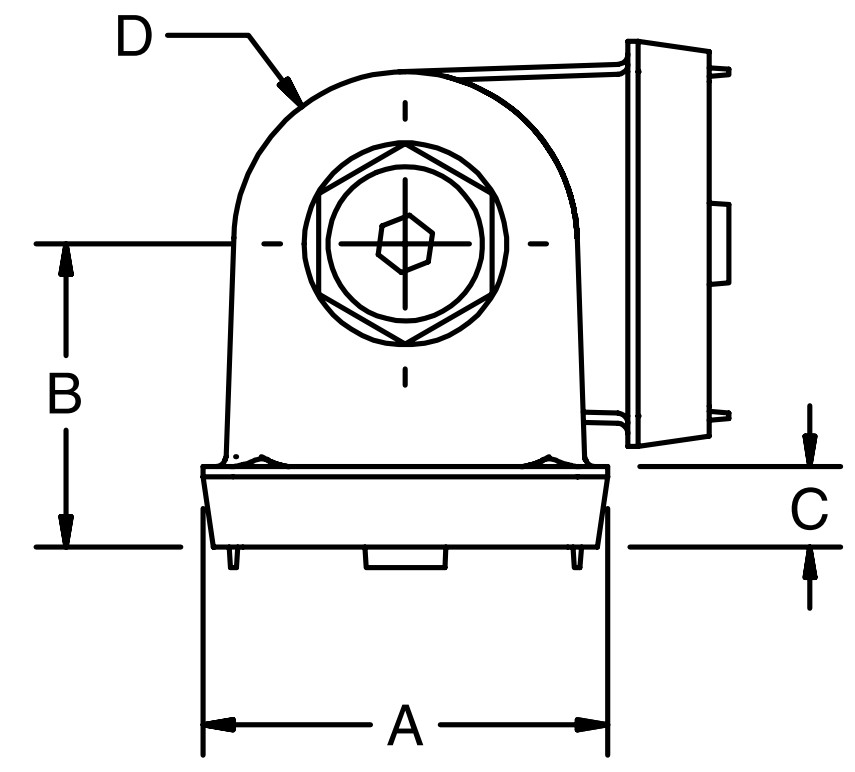
\includegraphics[width=4cm]{pivotjoint.jpg} \caption{}
    \end{subfigure}
	\begin{subfigure}{0.32\linewidth}
		\centering 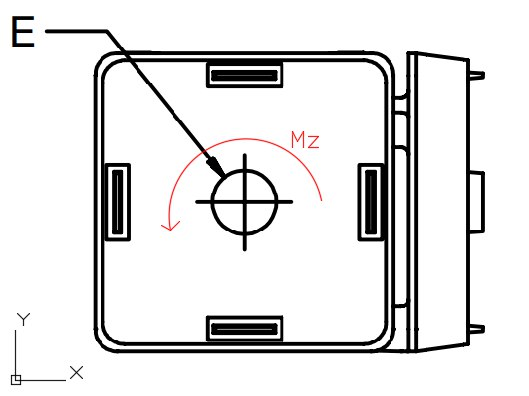
\includegraphics[width=4cm]{sectionD} \caption{}
	\end{subfigure}
	\begin{subfigure}{0.32\linewidth}
		\centering 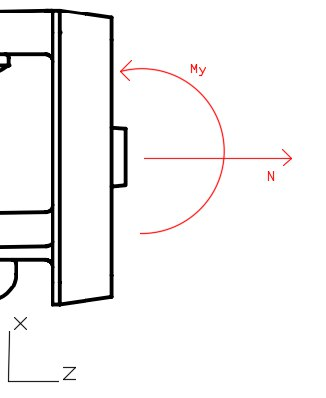
\includegraphics[width=3cm]{xz.png} \caption{}
	\end{subfigure}    
    \caption{pivot joint, code \texttt{23-010}, from the IPS catalogue \cite{parker-ds}. In the drawing: $A = 40mm$, $B=30mm$, $C=9mm$, $D=40mm$, $E=8.5mm$, $F=60mm$.}
    \label{fig:pivot}
\end{figure}

In this case, the sliding actions are given by the torque $M_{zD}$,  figure \ref{fig:pivot}\textit{(b)}. However, since there is a single screw positioned in the center of the section, they do not cause any shear on the screw. \textbf{(??)}

Separating actions are given by the axial load and the bending moments. Assuming that the members are rigid it is possible to calculate the effects of the separating actions in both $xz$ and $yz$ planes. The load caused by the separating action, acting on the screw can be calculated as:
\begin{equation*}
    N_{i} = \frac{M_{b}h_{i}}{\sum\limits_{i=1}^{n_{b}} h^2_{i}} + \frac{N}{n_{b}}
\end{equation*}\\
where $h_{i}$ is the distance of the $i$-th bolt from the pivot point.
\begin{equation*}
    N_{xz} = \frac{M_{yD}}{h} + N_{D} = 638.328 N
\end{equation*}

Considering the $xz$ plane and assuming the pivot on the edge of the section, $h$ is equal to $\frac{A}{2} = 20 mm$. The tension resistance and punching verification can be performed as follow:
\begin{itemize}
    \item tension resistance verification:
    \begin{equation*}
        N_{xz} < \frac{\sigma_{uts}A_{bt}}{\phi}
    \end{equation*}
    Where $\sigma_{uts}$ corresponds to the screw's ultimate tensile strength, $A_{bt}$ to the bolt tensile cross-section and $\phi$ is the safety factor which, according to Eurocode3, is equal to $\frac{1.25}{0.9}$. As a consequence, it follows that:
    \begin{equation*}
       \sigma_{uts} > \frac{N_{xz}\phi}{A_{bt}} = 24.223 MPa
    \end{equation*}
    \item punching resistance verification:
    \begin{equation*}
        N_{xz} < \frac{\pi d_{0} t \sigma_{uts,m}}{\phi}
    \end{equation*}
    Where $\sigma_{uts,m}$ corresponds to the member's ultimate tensile strength, $d_{0}$ the bolt head diameter and $\phi$ is the safety factor which, according to Eurocode3, is equal to $\frac{1.25}{0.6}$. Finally, $t$ corresponds to the member's thickness, which can be calculated as the sum of the pivot joint thickness, $C = 9 mm$, and the member's cross section, equal to $40 mm$:
     \begin{equation*}
       \sigma_{uts,m} > \frac{N_{xz}\phi}{\pi d_{0}t} = 0.617 MPa
    \end{equation*}
\end{itemize}
Considering instead the $xz$ plane we have:\\
\begin{equation*}
    N_{yz} = \frac{M_{xD}}{h} + N_{D} = 233.010 N
\end{equation*}
thus:
\begin{itemize}
    \item tension resistance verification:
    \begin{equation*}
        N_{yz} < \frac{\sigma_{uts}A_{bt}}{\phi} \qquad \Rightarrow \sigma_{uts} > \frac{N_{yz}\phi}{A_{bt}} = 8.842 MPa
    \end{equation*}
    \item punching resistance verification\\
    \begin{equation*}
        N_{yz} < \frac{\pi d_{0} t \sigma_{uts,m}}{\phi} \qquad \Rightarrow \qquad   \sigma_{uts,m} > \frac{N_{yz}\phi}{\pi d_{0}t} = 0.225 MPa
    \end{equation*}
\end{itemize}
In conclusion, the bolt ultimate strength must be greater than $24.223 MPa$, a value that allows to choose any bolt property class. In order to minimize the costs, property 4.6 is chosen.\textbf{(????)} 

Moreover, the verifications for crushing and punching provide the minimum member ultimate strength, $\sigma_{uts,m} > 0.226 MPa$, value much smaller than the chosen member's UTS.

Note that for the verifications of the separating actions the rigid member approach was used, which is usually more conservative than the others. However, since the values obtained are far distant from the one of the selected materials, there is no need of a more precise verification.